
%(BEGIN_QUESTION)
% Copyright 2011, Tony R. Kuphaldt, released under the Creative Commons Attribution License (v 1.0)
% This means you may do almost anything with this work of mine, so long as you give me proper credit

After years of trouble-free operation, several of the stack gas analyzers in this incinerator system begin to register zero or near-zero concentration levels.  The affected analyzers are those measuring hydrogen sulfide, acetylene, ammonia, nitric acid, and methane:

$$\includegraphics[width=15.5cm]{i0004rx01.eps}$$

Identify likely faults which could account for the analyzer problems in this system, and also describe a good diagnostic test you could perform to help isolate the fault(s).

\vskip 20pt \vbox{\hrule \hbox{\strut \vrule{} {\bf Suggestions for Socratic discussion} \vrule} \hrule}

\begin{itemize}
\item{} A useful assumption to make while diagnosing faults is that a single fault is more likely than multiple, coincidental faults.  Given this assumption (based on a philosophical proverb known as {\it Occam's Razor}), identify single points of failure that could account for all the bad analyzer indications described in the problem.
\end{itemize}

\underbar{file i03363}
%(END_QUESTION)





%(BEGIN_ANSWER)

 
%(END_ANSWER)





%(BEGIN_NOTES)

\vskip 20pt \vbox{\hrule \hbox{\strut \vrule{} {\bf Virtual Troubleshooting} \vrule} \hrule}

This question is a good candidate for a ``Virtual Troubleshooting'' exercise.  Presenting the diagram to students, you first imagine in your own mind a particular fault in the system.  Then, you present one or more symptoms of that fault (something noticeable by an operator or other user of the system).  Students then propose various diagnostic tests to perform on this system to identify the nature and location of the fault, as though they were technicians trying to troubleshoot the problem.  Your job is to tell them what the result(s) would be for each of the proposed diagnostic tests, documenting those results where all the students can see.

During and after the exercise, it is good to ask students follow-up questions such as:

\begin{itemize}
\item{} What does the result of the last diagnostic test tell you about the fault?
\item{} Suppose the results of the last diagnostic test were different.  What then would that result tell you about the fault?
\item{} Is the last diagnostic test the best one we could do?
\item{} What would be the ideal order of tests, to diagnose the problem in as few steps as possible?
\end{itemize}

%INDEX% Basics, control loop troubleshooting (realistic P&ID shown)
%INDEX% Measurement, analytical: sample conditioning
%INDEX% Process: incinerator (realistic P&ID shown)

%(END_NOTES)


